\documentclass[11pt]{article}
\usepackage[preprint]{acl}
\usepackage{times}
\usepackage{latexsym}
\usepackage[T1]{fontenc}
\usepackage[utf8]{inputenc}
\usepackage{microtype}
\usepackage{graphicx}
\usepackage{booktabs}
\title{Separating Evidence, Memory, and Programs in Annotation-Policy Adaptation:\\Protocol and Preliminary Controls}
\author{Research Working Draft\\Authors to be confirmed}
\begin{document}
\maketitle
\begin{abstract}
Annotation manuals specify categories and conventions, but examples may be needed to operationalize them. We develop an evaluation protocol for fixed-weight agents that retrieve guidelines and examples, maintain natural-language notes, and modify executable annotation programs. The central question is whether different persistent representations improve transfer under matched annotation and feedback budgets. We audit linguistic, political-text, and visual annotation resources, identifying confounds involving segmentation, perception, versioning, and hidden annotation fields. We implement metered evidence access, frozen evaluation states, and isolated program execution. As a completed preliminary control experiment, we evaluate three non-LLM methods on 485 SNACS targets in the official STREUSLE test split, using four annotation budgets and five paired adaptation trajectories. With 128 labeled sentences, lexical majority achieves 32.66\% joint accuracy and TF--IDF nearest-example prediction achieves 25.03\%. These controls do not establish agent learning or an advantage of self-modification. Model experiments and cross-domain results are not yet available because inference and dataset prerequisites remain unresolved.
\end{abstract}

\noindent\fbox{\parbox{0.94\columnwidth}{\textbf{Preliminary empirical working paper.} The requested full agent study is incomplete. All numerical results come from completed non-LLM controls. No model results, human annotations, or expert gap findings have been fabricated.}}

\section{Research Question}
An annotator may understand a label definition yet remain uncertain about its application to a particular construction. A motivating observation from Uniform Meaning Representation concerns occupational roles expressed through apposition. This is a hypothesis about an operational gap, not an established omission in the official manual: related role predicates already appear in public documentation, and failure may instead reflect scattered rules or difficulty applying them.

We study \emph{annotation-policy adaptation}: how a fixed-weight system uses newly revealed annotations to improve decisions under a specified convention. The question is not whether machine learning can read guidelines. Guideline-conditioned extraction already exists, for example in GoLLIE \citep{gollie}. Nor is iterative guideline refinement itself novel. \citet{kim2026refining} directly studies guideline reuse, refinement, minimal supervision, and model differences on biomedical named-entity recognition.

Our proposed comparison isolates persistent external state: original examples, refined natural-language policy, and executable annotation programs. We ask when these representations help unseen instances or constructions, how much additional annotation they require, and whether policy changes make earlier adaptations harmful. These remain research questions rather than established findings.

\section{Related Work and Novelty Boundary}
GuideBench evaluates domain-oriented rules and updates \citep{guidebench}. The closest identified annotation work is \citet{kim2026refining}; its official abstract describes iterative moderation on NCBI Disease, BC5CDR, and BioRED with three model families. A reproduction on one accessible dataset is a required calibration step, followed by a budget-matched refinement baseline.

This literature audit verifies official abstracts and selected project documentation, not every full paper. We do not claim that previous work lacks all proposed analyses, or that ours is the first self-improving annotation agent. Before submission, full-text comparisons, implementation details and bibliographic metadata must be verified. The intended contribution is controlled evidence about transfer and failure mechanisms, not a recombination of retrieval, memory, and code generation.

\section{Cross-Domain Benchmark Audit}
\paragraph{Linguistic annotation.}
UMR offers semantic graphs; SNACS distinguishes scene role from lexical function; GUM/DISRPT offers discourse relations; UD EWT offers candidate natural policy revisions. These remain concentrated in linguistic annotation. STREUSLE and UD EWT share review texts, so they cannot count as independent corpora. Relation classification with supplied discourse units is not full discourse parsing.

Official resources expose two evaluator hazards. UD LAS ignores relation subtypes, requiring full-label or phenomenon-specific measures for changes such as \texttt{nmod:desc}. DISRPT files may include an original fine-grained gold label as well as the target label; deleting only the final column does not remove the answer.

\paragraph{Manifesto.}
Manifesto extends the scope to political-text coding \citep{manifesto}. The required resource is the coded quasi-sentence Corpus, not party--election aggregate statistics. We propose a first track with supplied official segmentation, fixed unlabeled context, one handbook version and one language. Documents, translations and near duplicates must be grouped across splits. Political knowledge, segmentation, country, election year and handbook changes cannot all vary and then be interpreted as a single policy-learning effect.

The official client distinguishes condensed codebook descriptions from the complete handbook. Its v5-to-v4 mapping contains exceptions, so truncating decimal codes is incorrect. Neither the inspected official repository nor the current CRAN package bundles a substitute sentence-level corpus. Corpus access requires an API key or legitimate export. The complete handbook, terms and actual corpus remain pending in this environment.

\paragraph{Fashionpedia.}
Fashionpedia supplies localized garment categories and attributes \citep{fashionpedia}. We propose a given-region category/attribute track, separating end-to-end segmentation. Supplied regions reduce localization demands but do not remove perception and fashion knowledge as confounds.

Official documentation lists 46 categories and 294 attributes. The API's two-image test sample has 48 categories and 320 attributes and explicitly warns that it is not final data. We do not use it for empirical claims. Taxonomy names and hierarchy are not a complete annotation manual; absent attribute entries are not automatically evidence of visual absence.

Official joint AP combines localization and attribute criteria with a specified attribute-F1 implementation. Our proposed supplied-region accuracy and multilabel F1 would be research diagnostics, not official joint AP. Annotation/ontology licenses must be distinguished from source-specific image rights. Full annotations and actual images have not yet been acquired here.

\section{Evaluation Protocol}
\subsection{Information and State}
The trusted controller owns raw gold, budgets and scoring. Models access versioned guideline fragments and purchased examples through bounded tools. They may persist notes; a separate condition may write standard-library Python programs. They cannot change the evaluator or purchase labels without recording them.

Supervision is measured as revealed examples, with additional counts of labeled decisions and guideline-embedded examples. Repeated reads consume compute but do not increase the unique-example count. One SNACS example is a sentence revealing all retained target labels. Gold target spans are additional structural supervision shared by all conditions.

At evaluation, every instance starts with the same frozen asset snapshot. Programs execute with read-only assets, cleared environment, isolated process/network namespaces, bounded CPU/output and no mounted repository or gold. An actual sentinel-file, environment and network test verified this isolation. There is no unrestricted fallback.

\subsection{Conditions and Identification}
Paired conditions are frozen retrieval, persistent guideline refinement, and refinement plus program modification. Frozen systems retain all the same purchased examples and fixed structural checks. Full-context prompting, when feasible, controls for tool-mediated access. Active selection is a separate experiment: choosing evidence and using evidence answer different questions.

We distinguish output validity, semantic correctness, transfer and cost. A code change that only improves serialization does not demonstrate semantic learning. Oracle relevant evidence diagnoses retrieval failures. Strong/weak-model asset exchange can help distinguish asset construction from execution, with teacher costs counted and hidden teacher calls prohibited.

\subsection{Sample Efficiency and Generalization}
We would predefine a quality target and report the smallest measured additional-label budget reaching it with stated uncertainty. An unreached target is a censored outcome, not permission to extrapolate an exact sample requirement. Learning-curve area uses a shared $\log_2(1+B)$ interval, defined at zero budget.

Public manuals and examples may occur in pretraining. We measure additional deployment-time supervision, not from-scratch sample complexity. Unseen-construction claims require auditing all authorized examples; a random split only establishes unseen-instance evaluation. Expert-designed new conventions and policy revisions offer diagnostics, not contamination guarantees.

\section{Completed Control Experiment}
\subsection{Data and Setup}
We pin STREUSLE \citep{streusle} to commit \texttt{8ba61fe4} (full SHA in the repository). Files are downloaded with TLS verification and SHA-256 provenance. We project official JSON into text, tokens and supplied target spans, removing syntax, MISC and other gold layers from predictor inputs. The scorer holds role/function pairs separately.

The training projection has 1,911 sentences, 4,553 retained target decisions and 347 documents. Development has 267 sentences, 462 targets and 156 documents. Test has 259 sentences, 485 targets and 146 documents. Document sets are disjoint. These counts describe our supplied-target projection, not all STREUSLE lexical annotations. Label validity uses the pinned official ontology rather than test-observed labels.

Budgets are 4, 16, 64 and 128 sentences, with seeds 11, 23, 47, 83 and 101. Each seed defines a shuffled nested training sequence shared across methods. Settings were recorded before generating test predictions. These controls do not access a guideline, invoke an LLM or modify programs.

\subsection{Methods and Metrics}
\textbf{Majority} predicts the most frequent observed joint role/function pair. \textbf{Lexical majority} uses the most frequent pair for the target expression, backing off to global majority. \textbf{TF--IDF nearest} marks target tokens, represents target and sentence with word unigram/bigram TF--IDF fit only to purchased inputs, and copies the nearest purchased target's pair. Zero similarity backs off to majority.

The primary metric is exact joint role/function accuracy over retained targets. We also save marginal accuracy, macro-F1, sentence exact match and ontology-valid output rate. The three marginal/joint accuracies and target denominators match the unmodified pinned official scorer for all 60 valid supplied-target runs; this does not establish equivalence for arbitrary invalid or auto-identification outputs. Gold self-scoring reaches 1.0; empty predictions reach 0.0. Predictors are tested without any test-gold field.

\subsection{Results}
\begin{table}[t]
\centering\small
\begin{tabular}{rccc}
\toprule
Budget & Majority & Lexical & TF--IDF \\\midrule
4 & 4.70 $\pm$ 6.06 & 6.52 $\pm$ 6.14 & 4.08 $\pm$ 0.78 \\
16 & 5.11 $\pm$ 1.19 & 11.26 $\pm$ 2.85 & 11.51 $\pm$ 2.76 \\
64 & 12.82 $\pm$ 4.98 & 27.38 $\pm$ 5.00 & 21.28 $\pm$ 3.18 \\
128 & 15.05 $\pm$ 0.00 & 32.66 $\pm$ 3.65 & 25.03 $\pm$ 1.72 \\
\bottomrule
\end{tabular}

\caption{Completed non-LLM controls: joint accuracy (\%) as mean $\pm$ adaptation-run standard deviation over five paired trajectories. Standard deviations are not confidence intervals.}
\label{tab:controls}
\end{table}
\begin{figure}[t]
\centering
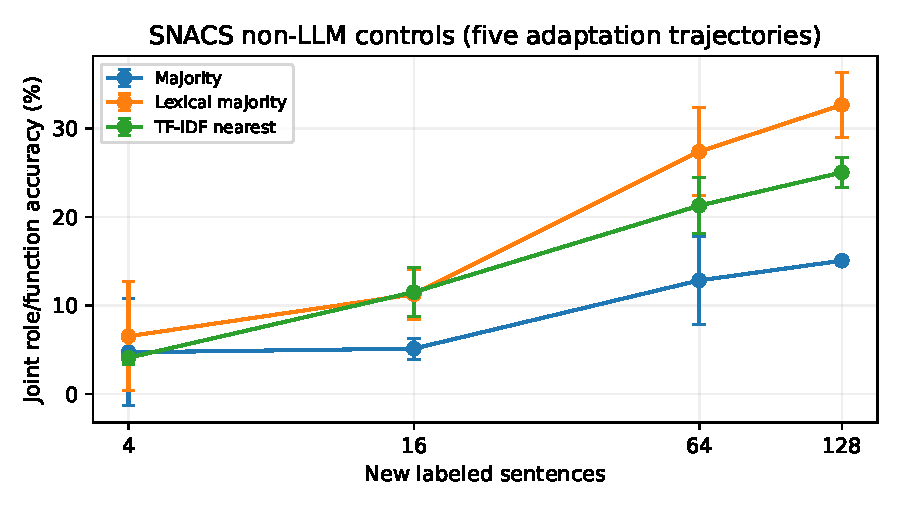
\includegraphics[width=\columnwidth]{control-learning-curves.pdf}
\caption{Measured controls. Error bars describe adaptation-trajectory variation; no agent curve is implied.}
\end{figure}

Table~\ref{tab:controls} reports all 60 runs without seed selection. At 128 sentences, lexical majority reaches 32.66\% versus 25.03\% for TF--IDF nearest, a paired difference of 7.63 percentage points. A descriptive two-axis bootstrap over paired trajectories and test documents yields a 95\% percentile interval of 3.62--11.48 points (2,000 resamples). Five trajectories provide limited evidence: this is not an agent hypothesis test or a general effect estimate.

A sentence is not a fixed amount of supervision: four purchased sentences reveal 6--10 target decisions across these trajectories; 128 reveal 269--308. This motivates multi-unit budget accounting, not a universal sample requirement. The relative strength of lexical majority also motivates retaining lexical controls rather than assuming general sentence-similarity retrieval is sufficient. It does not demonstrate superiority over neural retrieval or parsing.

\section{Implementation Review and Pending Work}
Three AI reviewers examined contribution, validity and resources, followed by code review. They are not human annotators or actual conference reviewers. Code review found malformed-completion handling, invalid-label validity scoring, and truncated-response usage loss. We fixed these issues and added regression coverage. All 60 prediction hashes remained unchanged after these fixes.

Ten unit/regression tests and a real isolation test passed. Model stubs appear only in software tests. Model experiments have \emph{not} run: a logged-in Codex inference probe was rejected by the network proxy; no model API binding or GPU was found. Official Manifesto and Fashionpedia data prerequisites also remain unresolved. Saved network drafts do not establish applied access.

The next empirical stage requires full version-aligned materials, closest-work reproduction, a reproducible inference backend, paired model runs and expert audits. Supplied-unit/region tracks should precede end-to-end evaluations, allowing segmentation and perception to be analyzed separately.

\section{Limitations}
This is not the complete requested agent study. It contains one genuine non-LLM experiment and a research protocol. There are no agent learning curves, model-strength comparisons, visual/political predictions or human sample-efficiency measurements. Guideline gaps have not been established by experts. Public contamination is unknown. A material-manifest gate is not scientific certification, and full-text literature comparison remains pending.

Five trajectories on one English dataset cannot establish general annotation-learning boundaries. Supplied targets remove part of the full task. Exact gold agreement may penalize reasonable alternatives, requiring adjudication. Manifesto and Fashionpedia broaden candidate scope, but neither provides evidence for the central hypothesis before real controlled experiments.

\section*{Ethical and Reproducibility Considerations}
We retain source hashes, split IDs, predictions and settings while avoiding redistribution of raw licensed texts or images. Credentials are not stored in source, results or manuscript. Dataset and software licenses are distinguished. Political-text gold is not treated as a universal definition of political meaning. Later human studies require appropriate consent, compensation and review. AI assistance in design, software and this draft is disclosed; expert adjudication has not been simulated.

\bibliography{references}
\end{document}
